\subsection{Seriel kommunikation}
De dette afsnit er der kun medtaget de mest nødvendige test, for alle øvrige tests henvises til dokumentation (reference til test under seriel kommunikation. 

\subsubsection{DevKit8000-PSoC Master}
På figur \ref{LA_SPI_1} ses resulater på Logic Analyzer når der skrives til PSoC master fra terminalen på Devkit8000.

\begin{figure}[H]
	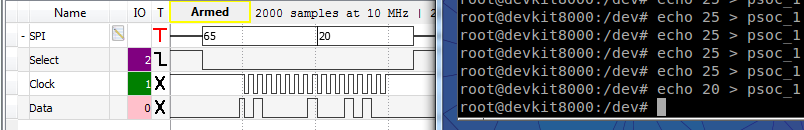
\includegraphics[scale=0.6]{tex/TeImRe/SPI/Analog_devkit_echo_psoc_1}
	\caption{Udskrift fra Logic Analyzer fra test af SPI forbindelse mellem Devkit og PSoC Master}
	\label{LA_SPI_1}
\end{figure}

Resultater for læsningen af PSoC Master gav kun succesfuldt resultater ved en enkelt test. Derudover kunne der ikke læses fra PSoC master
Hvilket betyder at der ikke er dokumentet en succesfuld aflæsning af MISO forbindelsen. Selv efter mange forsøg, og med hjælp fra undervisere i HAL, blev 
dette problem aldrig løst.

\subsubsection{PSoC Master - PSoC Slave}
På figur \ref{LA_SPI_3} ses udskrift Logic Analyzer og PC Terminal. Der er i denne test blevet skrevet værdien 5 til PSoC slave. Billeder for test af MISO er udeladt, men
gav dog samme resultat.

\begin{figure}[H]
	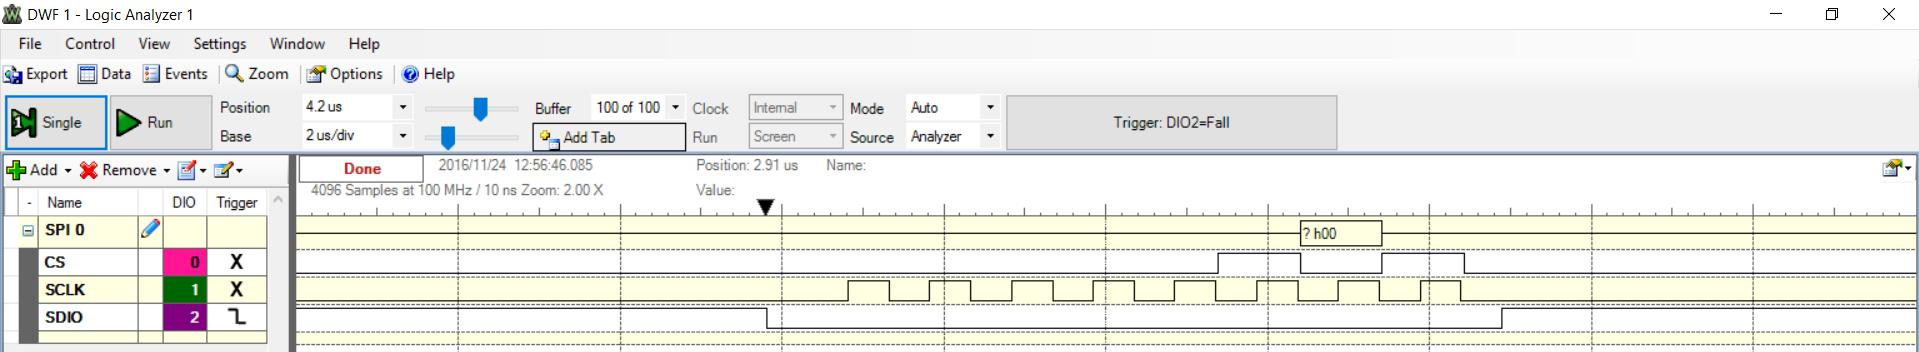
\includegraphics[scale=0.2]{tex/TeImRe/SPI/Logic_analyzer}
	\caption{Udskrift fra Logic Analyzer fra test af SPI forbindelse mellem PSoC Slave og PSoC Master}
	\label{LA_SPI_2}
\end{figure}

\begin{figure}[H]
	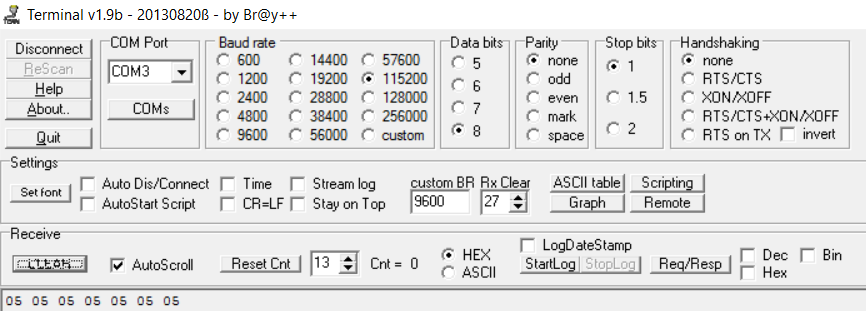
\includegraphics[scale=0.4]{tex/TeImRe/SPI/Terminal_spi_slave}
	\caption{Udskrift fra terminal fra test af SPI forbindelse mellem PSoC Slave og PSoC Master}
	\label{LA_SPI_3}
\end{figure}